% !TeX program = xelatex
% Compile twice with XeLaTeX.
\documentclass[12pt,a4paper,oneside]{report}
\XeTeXgenerateactualtext=1
\usepackage[margin=22mm,top=24mm,bottom=24mm,headheight=27pt]{geometry}
\usepackage{amsmath,amssymb,mathtools,bm}
\usepackage{booktabs,array,longtable,tabularx,graphicx}
\usepackage[table]{xcolor}
\usepackage{tikz}
\usetikzlibrary{arrows.meta,calc,patterns,positioning}
\usepackage[most]{tcolorbox}
\usepackage{titlesec,needspace}
\usepackage{hyperref}
\usepackage{bookmark}
\usepackage{enumitem}
\usepackage{xepersian}
\settextfont[Scale=1.06,BoldFont=Amiri-Bold.ttf]{Amiri-Regular.ttf}
\setlatintextfont[BoldFont=texgyretermes-bold.otf,ItalicFont=texgyretermes-italic.otf,BoldItalicFont=texgyretermes-bolditalic.otf]{texgyretermes-regular.otf}

%%% ─── پالت رنگی هماهنگ و چشم‌نواز ───
\definecolor{navy}{HTML}{163747}      % رنگ اصلی عناوین
\definecolor{teal}{HTML}{127C80}      % رنگ زیرعنوان‌ها و نمادها
\definecolor{gold}{HTML}{B18542}      % رنگ کادرهای یادآوری
\definecolor{paper}{HTML}{F8FAFA}     % پس‌زمینه لطیف کادرها
\definecolor{muted}{HTML}{5E7178}     % رنگ متن‌های راهنما
\definecolor{solframe}{HTML}{2B6CB0}  % حاشیه کادر حل تمرین
\definecolor{solbg}{HTML}{F0F6FC}    % پس‌زمینه کادر حل تمرین
\definecolor{stepcolor}{HTML}{0D5C75} % رنگ تیتر گام‌ها
\definecolor{notecolor}{HTML}{B07D2B} % رنگ نکات درون حل
\definecolor{resframe}{HTML}{238636}  % رنگ کادر نتیجه
\definecolor{resbg}{HTML}{F2F9F3}     % پس‌زمینه کادر نتیجه

\hypersetup{unicode=true,colorlinks=true,linkcolor=navy,urlcolor=teal,
 pdftitle={روش‌های آماری ـ مرور جلسه اول},pdfauthor={علیرضا جهانبخش و احسان شهبازی},pdfsubject={مقدمات، نااریبی، کارایی، سازگاری}}
\setlength{\parindent}{0pt}
\setlength{\parskip}{5pt plus 1pt}
\linespread{1.14}
\raggedbottom
\setcounter{tocdepth}{1}
\setcounter{secnumdepth}{2}
\allowdisplaybreaks[2]
\emergencystretch=1em

%%% ─── سربرگ و پانویس ───
\makeatletter
\def\ps@lecture{%
  \def\@oddhead{\vbox{\hbox to\textwidth{\small
    \rl{روش‌های آماری}\hfil\rl{\leftmark}}%
    \kern4pt\hrule height .35pt}}%
  \let\@evenhead\@oddhead
  \def\@oddfoot{\hfil\thepage\hfil}%
  \let\@evenfoot\@oddfoot}
\makeatother
\pagestyle{lecture}
\renewcommand{\chaptermark}[1]{\markboth{#1}{}}
\titleformat{\chapter}[display]{\color{navy}\bfseries\Huge}{\large فصل \thechapter}{8pt}{}[\vspace{4pt}\color{gold}\titlerule]
\titlespacing*{\chapter}{0pt}{0pt}{18pt}
\titleformat{\section}{\Large\bfseries\color{navy}}{\thesection}{.6em}{}
\titleformat{\subsection}{\large\bfseries\color{teal}}{\thesubsection}{.6em}{}

%%% ─── استایل یکدست و استاندارد باکس‌ها ───
\tcbset{enhanced,breakable,boxrule=.6pt,arc=2mm,
 left=4mm,right=4mm,top=3mm,bottom=3mm,before skip=8pt,after skip=8pt,
 fonttitle=\bfseries,coltitle=white}

% ۱. تعریف و صورت مفاهیم
\newtcolorbox{definition}[1]{title={تعریف | #1},colframe=navy,colback=navy!3!white}

% ۲. صورت سوال و مسئله
\newtcolorbox{question}[1][صورت مسئله]{title={#1},colframe=navy,colback=navy!2!white}

% ۳. کادر حل (یکپارچه برای تمام مثال‌ها و تمرین‌ها)
\newtcolorbox{solutionbox}[1][راه حل تشریحی]{title={#1},colframe=solframe,colback=solbg}

% ۴. یادآوری و پیش‌نیازها
\newtcolorbox{reminder}[1][]{title={یادآوری #1},colframe=gold,colback=gold!6!white}

% ۵. نتیجه کلیدی
\newtcolorbox{result}[1]{title={نتیجهٔ کلیدی | #1},colframe=resframe,colback=resbg}

%%% ─── دستورات کمکی داخل باکس حل ───
\newcommand{\step}[1]{\par\smallskip\noindent\textbf{\color{stepcolor}$\blacktriangleleft$ #1}\par\smallskip}
\newcommand{\substep}[1]{\par\noindent\textbf{\color{teal}• #1:}\ }
\newcommand{\notein}[1]{\par\smallskip\noindent{\color{notecolor}\textbf{نکته کلاسی:} #1}\par}
\newcommand{\problem}[2]{\Needspace{9\baselineskip}\section*{تمرین #1: #2}\addcontentsline{toc}{section}{تمرین #1: #2}}

%%% ─── کادر یادداشت نیم‌صفحه برای دانشجویان ───
\newcommand{\notespace}{%
  \par\vspace{8pt}%
  \begin{tcolorbox}[breakable=false,colback=white,colframe=muted!50,boxrule=.6pt,arc=1.5mm,height=0.36\textheight]
    \textcolor{muted!70}{\small\textbf{محل یادداشت‌ها و نکات تکمیلی دانشجو / \lr{TA}:}}
  \end{tcolorbox}%
  \par\vspace{8pt}%
}

%%% ─── نمادهای آماری ───
\newcommand{\E}{\mathbb E}
\newcommand{\Var}{\operatorname{Var}}
\newcommand{\Cov}{\operatorname{Cov}}
\newcommand{\MSE}{\operatorname{MSE}}
\newcommand{\Bias}{\operatorname{Bias}}
\newcommand{\SE}{\operatorname{SE}}
\newcommand{\iid}{\overset{\mathrm{iid}}{\sim}}
\newcommand{\N}{\mathcal N}
\newcommand{\R}{\mathbb R}
\newcommand{\Prob}{\mathbb P}

\begin{document}

%%% ═══════════════════════════════════════════════════
%%%  صفحهٔ جلد
%%% ═══════════════════════════════════════════════════
\begin{titlepage}
\begin{tikzpicture}[remember picture,overlay]
\fill[navy] (current page.north west) rectangle ([yshift=-90mm]current page.north east);
\fill[gold] ([yshift=-90mm]current page.north west) rectangle ([yshift=-92mm]current page.north east);
\draw[teal!22,line width=.5pt] ([xshift=23mm,yshift=32mm]current page.south west)--([xshift=-23mm,yshift=32mm]current page.south east);
\end{tikzpicture}
\vspace*{5mm}
\begin{center}
\textcolor{white}{{\large جزوه و راهنمای حل تمرین}}\\[12mm]
\textcolor{white}{{\fontsize{36}{46}\selectfont\bfseries روش‌های آماری}}\\[5mm]
\textcolor{white!85!navy}{{\Large جلسهٔ اول: مقدمات و برآورد نقطه‌ای}}
\end{center}
\vspace{12mm}
\begin{center}
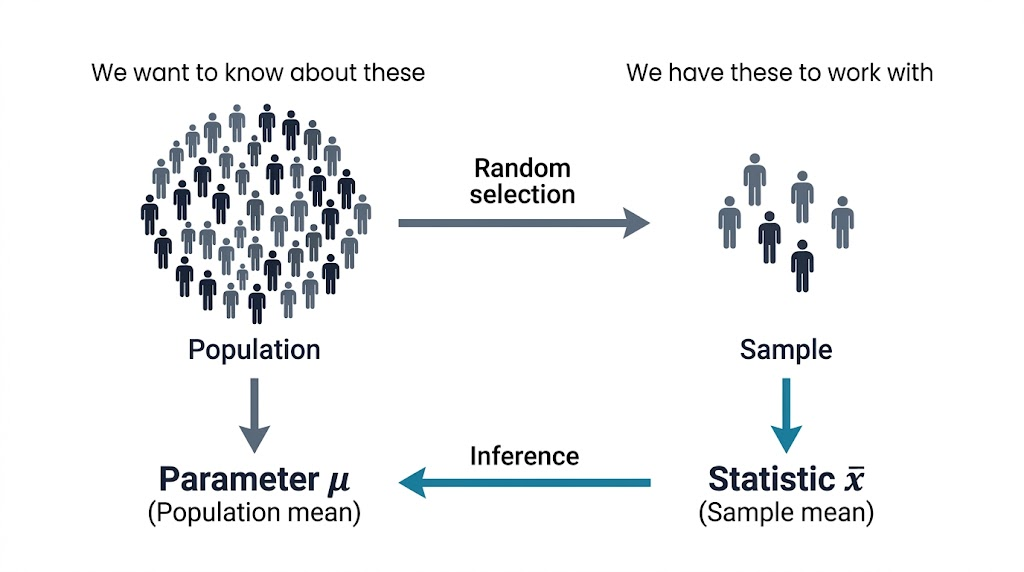
\includegraphics[width=0.70\textwidth]{inference_cover.png}\\[6mm]
{\large مرور توزیع‌ها و امید ریاضی \quad | \quad مفهوم برآورد نقطه‌ای}\\[4mm]
{\large نااریبی \quad | \quad کارایی \quad | \quad سازگاری}\\[12mm]
{\color{teal}\large درس‌نامهٔ جامع به‌همراه مثال‌ها و تمرین‌های حل‌شده با بیان مفهومی و گام‌به‌گام}\\[8mm]
{\color{navy}\large\textbf{استاد درس: دکتر سکینه دهقان}}\\[4mm]
{\color{navy}\large گردآورندگان حل تمرین: علیرضا جهانبخش و احسان شهبازی}
\end{center}
\vfill
\end{titlepage}

\pagenumbering{roman}
\tableofcontents
\clearpage\pagenumbering{arabic}

%%% ═══════════════════════════════════════════════════
%%%  فصل اول: مقدمات
%%% ═══════════════════════════════════════════════════
\chapter*{فصل اول: مقدمات و مرور پایه‌ها}
\markboth{مقدمات و مرور پایه‌ها}{}
\addcontentsline{toc}{chapter}{فصل اول: مقدمات و مرور پایه‌ها}

سلام به همهٔ دوستان عزیز دانشجوی کارشناسی آمار! به اولین جلسه از حل تمرین درس شیرین و پایه‌ای «روش‌های آماری» خیلی خوش اومدید. 

قبل از اینکه وارد بحث اصلی برآورد نقطه‌ای بشیم، برای اینکه دستمون توی فرمول‌ها و امید ریاضی‌ها گرم بشه، تو این بخش اول خیلی سریع فرمول‌های طلایی توزیع‌های پرکاربرد و خواص حیاتی امید ریاضی و واریانس رو دوره می‌کنیم و بعد فلسفهٔ این رو بررسی می‌کنیم که اصلاً «برآورد نقطه‌ای» چیه و قراره چه مشکلی رو برامون حل کنه!

\section*{۱. مرور توزیع‌های پرکاربرد آماری}
\addcontentsline{toc}{section}{۱. مرور توزیع‌های پرکاربرد آماری}

در روابط زیر قرارداد می‌کنیم $q = 1 - p$.

\Needspace{5\baselineskip}\textbf{\textcolor{navy}{۱. توزیع برنولی ($X \sim \operatorname{Bernoulli}(p)$):}}
مدلِ یک بار پرتاب سکه یا یک آزمایش با دو نتیجهٔ موفقیت (۱) و شکست (۰).
\[
p_X(x) = p^x (1-p)^{1-x} \quad (x \in \{0, 1\}), \qquad \E(X) = p, \qquad \Var(X) = p(1-p).
\]

\Needspace{5\baselineskip}\textbf{\textcolor{navy}{۲. توزیع دوجمله‌ای ($X \sim \operatorname{Bin}(n, p)$):}}
تعداد موفقیت‌ها در $n$ آزمایش مستقل و هم‌شانس برنولی.
\[
p_X(x) = \binom{n}{x} p^x (1-p)^{n-x} \quad (x = 0, 1, \dots, n), \qquad \E(X) = np, \qquad \Var(X) = np(1-p).
\]

\Needspace{5\baselineskip}\textbf{\textcolor{navy}{۳. توزیع پواسون ($X \sim \operatorname{Poisson}(\lambda)$):}}
شمارش تعداد پیشامدهای نادر در یک بازهٔ زمانی یا مکانی مشخص با نرخ $\lambda > 0$.
\[
p_X(x) = \frac{\lambda^x e^{-\lambda}}{x!} \quad (x = 0, 1, 2, \dots), \qquad \E(X) = \lambda, \qquad \Var(X) = \lambda.
\]

\Needspace{5\baselineskip}\textbf{\textcolor{navy}{۴. توزیع یکنواخت پیوسته ($X \sim U(a, b)$):}}
شانس کاملاً برابر روی بازهٔ پیوستهٔ $(a, b)$.
\[
f_X(x) = \frac{1}{b-a} \quad (a < x < b), \qquad \E(X) = \frac{a+b}{2}, \qquad \Var(X) = \frac{(b-a)^2}{12}.
\]

\Needspace{5\baselineskip}\textbf{\textcolor{navy}{۵. توزیع نمایی ($X \sim \operatorname{Exp}(\lambda)$):}}
طول زمان انتظار تا وقوع اولین پیشامد با نرخ رخداد $\lambda > 0$.
\[
f_X(x) = \lambda e^{-\lambda x} \quad (x > 0), \qquad \E(X) = \frac{1}{\lambda}, \qquad \Var(X) = \frac{1}{\lambda^2}.
\]

\Needspace{5\baselineskip}\textbf{\textcolor{navy}{۶. توزیع نرمال ($X \sim \mathcal{N}(\mu, \sigma^2)$):}}
پادشاه توزیع‌های احتمال در طبیعت و آمار، متقارن حول میانگین.
\[
f_X(x) = \frac{1}{\sigma\sqrt{2\pi}} \exp\!\left(-\frac{(x-\mu)^2}{2\sigma^2}\right) \quad (x \in \R), \qquad \E(X) = \mu, \qquad \Var(X) = \sigma^2.
\]

\Needspace{5\baselineskip}\textbf{\textcolor{navy}{۷. توزیع گاما ($X \sim \operatorname{Gamma}(\alpha, \lambda)$):}}
با پارامتر شکل $\alpha > 0$ و نرخ $\lambda > 0$.
\[
f_X(x) = \frac{\lambda^\alpha}{\Gamma(\alpha)} x^{\alpha-1} e^{-\lambda x} \quad (x > 0), \qquad \E(X) = \frac{\alpha}{\lambda}, \qquad \Var(X) = \frac{\alpha}{\lambda^2}.
\]

\notespace

\clearpage
\section*{۲. مرور امید ریاضی و خواص کلیدی آن}
\addcontentsline{toc}{section}{۲. مرور امید ریاضی و خواص کلیدی آن}

\begin{definition}{امید ریاضی \lr{(Expected Value)}}
امید ریاضی یک متغیر تصادفی $X$ که با نماد $\E(X)$ یا $\mu$ نشون داده می‌شه، در واقع همون میانگین وزنیِ مقادیر ممکن متغیر برحسب احتمال وقوع اون‌هاست:
\[
\E(X) = \begin{cases}
\displaystyle\sum_x x\,p_X(x) & \text{اگر $X$ گسسته باشد} \\[10pt]
\displaystyle\int_{-\infty}^{+\infty} x\,f_X(x)\,dx & \text{اگر $X$ پیوسته باشد}
\end{cases}
\]
\end{definition}

امید ریاضی چند تا قانون و خاصیت معجزه‌آسا داره که در طول این ترم توی تک‌تک سوالات باهاشون سر و کار داریم:

\begin{reminder}[ـ خواص ابزاری و ضروری امید ریاضی، واریانس و کوواریانس]
فرض کنید $X$ و $Y$ دو متغیر تصادفی با گشتاورهای متناهی باشند و $a, b, c$ اعداد ثابت حقیقی باشند:
\begin{enumerate}[itemsep=4pt]
\item \textbf{خطی بودن امید ریاضی (خیلی مهم!):} امید ریاضی همیشه و بدون هیچ شرطی عملگر خطیه:
\[
\E(aX + bY + c) = a\E(X) + b\E(Y) + c
\]
حتی اگه $X$ و $Y$ به شدت به هم وابسته هم باشن، این رابطه باز هم برقراره!
\item \textbf{تعریف و رابطهٔ برگشتی واریانس:}
\[
\Var(X) = \E(X^2) - [\E(X)]^2 \quad\Longrightarrow\quad \E(X^2) = \Var(X) + [\E(X)]^2
\]
\item \textbf{واریانس تبدیل خطی:} $\Var(aX + b) = a^2 \Var(X)$. (عدد ثابت $b$ تاثیری روی پراکندگی نداره).
\item \textbf{تعریف و رابطهٔ کوواریانس:}
\[
\Cov(X, Y) = \E(XY) - \E(X)\E(Y) \quad\Longrightarrow\quad \E(XY) = \Cov(X, Y) + \E(X)\E(Y)
\]
\item \textbf{شرط استقلال:} اگر دو متغیر $X$ و $Y$ مستقل باشند، آنگاه $\Cov(X, Y) = 0$ است و در نتیجه:
\[
\E(XY) = \E(X)\E(Y) \qquad \text{و} \qquad \Var(X + Y) = \Var(X) + \Var(Y)
\]
\end{enumerate}
\end{reminder}

برای اینکه ببینیم چطور از خطی بودن امید ریاضی توی آمار استفاده می‌کنیم، یک مثال ساده اما حیاتی رو با هم حل کنیم:

\begin{question}[مثال کلاسی: امید ریاضی میانگین نمونه]
فرض کنید $X_1, X_2, \dots, X_n$ یک نمونهٔ تصادفی از جامعه‌ای با میانگین $\mu$ باشند (یعنی $\E(X_i) = \mu$). امید ریاضی میانگین نمونه، یعنی $\bar{X} = \frac{1}{n}\sum_{i=1}^n X_i$ را به دست آورید.
\end{question}

\begin{solutionbox}
بیایید مرحله به مرحله با هم پیش بریم:

\step{گام اول: نوشتن تعریف میانگین نمونه}
میانگین نمونه تعریفش اینه که همهٔ داده‌ها رو جمع کنیم و تقسیم بر تعداد ($n$) کنیم:
\[
\bar{X} = \frac{1}{n}(X_1 + X_2 + \dots + X_n)
\]

\step{گام دوم: اعمال امید ریاضی و استفاده از خاصیت خطی بودن}
حالا از دو طرف تساوی بالا امید ریاضی می‌گیریم. چون ضریب $\frac{1}{n}$ یک عدد ثابت هست، خیلی راحت از داخل امید ریاضی میاد بیرون:
\[
\E(\bar{X}) = \E\!\left(\frac{1}{n}\sum_{i=1}^n X_i\right) = \frac{1}{n} \E\!\left(\sum_{i=1}^n X_i\right)
\]
حالا از خاصیت خطی بودن استفاده می‌کنیم؛ امید ریاضیِ یک جمع، تبدیل می‌شه به جمعِ امید ریاضی‌ها:
\[
\E(\bar{X}) = \frac{1}{n} \sum_{i=1}^n \E(X_i)
\]

\step{گام سوم: جایگذاری امید ریاضی هر متغیر}
چون تمام مشاهدات از یک جامعه اومدن، امید ریاضی تک‌تک اون‌ها برابره با $\mu$:
\[
\E(\bar{X}) = \frac{1}{n} \Big( \underbrace{\mu + \mu + \dots + \mu}_{\text{به تعداد $n$ بار}} \Big) = \frac{1}{n} (n\mu) = \mu
\]

\notein{دیدید چقدر سرراست بود؟ این نتیجه به ما می‌گه میانگین حسابیِ نمونه، به‌طور متوسط دقیقاً مساوی میانگین واقعی جامعه یعنی $\mu$ است!}
\end{solutionbox}

\notespace

\clearpage
\section*{۳. اصلاً «برآورد نقطه‌ای» یعنی چه؟}
\addcontentsline{toc}{section}{۳. اصلاً «برآورد نقطه‌ای» یعنی چه؟}

بیایید با یک مثال کاملاً ملموس از دانشگاه خودمون صحبت کنیم تا قضیه براتون شفاف بشه:

فرض کنید شما به عنوان پژوهشگر یا نمایندهٔ آموزش می‌خواید وضعیت تحصیلی و مشخصات دانشجویان \textbf{دانشکدهٔ ریاضی} رو بررسی کنید. جامعهٔ مورد نظر ما، کل دانشجویان دانشکدهٔ ریاضی هستن. توی این جامعه، سه تا ویژگی یا کمیت ناشناخته وجود داره که بهشون می‌گیم \textbf{پارامترهای جامعه}:
\begin{enumerate}[itemsep=3pt]
\item \textbf{میانگین جامعه ($\mu$):} مثلاً میانگین واقعی معدل کل تمام دانشجویان دانشکدهٔ ریاضی.
\item \textbf{واریانس جامعه ($\sigma^2$):} میزان پراکندگی یا نوسان نمرات دانشجوها حول این میانگین.
\item \textbf{نسبت جامعه ($p$):} مثلاً نسبت (درصد) دانشجویانی که در ترم اول نمرهٔ ریاضی عمومی ۱ رو بالای ۱۷ گرفتن.
\end{enumerate}

حالا مشکل کجاست؟ مشکل اینجاست که ما این پارامترهای واقعی ($\mu, \sigma^2, p$) رو \textbf{در اختیار نداریم}! اگر بخوایم مقدار دقیق این‌ها رو حساب کنیم، باید پروندهٔ تک‌تک چند صد یا چند هزار دانشجوی دانشکده رو باز کنیم، یا از تک‌تکشون بپرسیم، که این کار یا وقت‌گیره، یا هزینه‌بره، یا عملاً غیرممکنه.

\begin{center}
\begin{tikzpicture}[x=1cm,y=1cm]
\draw[thick,navy,fill=navy!5,rounded corners=8pt] (0,0) rectangle (4.6,2.8);
\node[navy,font=\bfseries] at (2.3,2.4) {\rl{جامعهٔ آماری}};
\node[font=\small,muted] at (2.3,1.8) {\rl{دانشجویان دانشکدهٔ ریاضی}};
\node[font=\small] at (2.3,1.1) {\rl{پارامترهای مجهول:}};
\node[font=\bfseries,teal] at (2.3,0.5) {$\mu \quad , \quad \sigma^2 \quad , \quad p$};

\draw[-{Latex[length=3mm]},line width=1.5pt,gold] (4.8,1.4) -- node[above,font=\small\bfseries,navy]{\rl{نمونه‌گیری تصادفی}} (7.4,1.4);

\draw[thick,teal,fill=teal!5,rounded corners=8pt] (7.6,0) rectangle (12.4,2.8);
\node[teal,font=\bfseries] at (10.0,2.4) {\rl{نمونهٔ آماری}};
\node[font=\small,muted] at (10.0,1.8) {\rl{مثلاً ۳۰ نفر دانشجو}};
\node[font=\small] at (10.0,1.1) {\rl{مشاهدات عددی:}};
\node[font=\bfseries,navy] at (10.0,0.5) {$X_1, X_2, \dots, X_n$};
\end{tikzpicture}
\end{center}

راه‌حل دنیای آمار چیه؟ می‌ریم یک نمونهٔ تصادفی مثلاً $n=30$ نفره از دانشجوها انتخاب می‌کنیم و معدل‌هاشون رو ثبت می‌کنیم: $X_1, X_2, \dots, X_n$. حالا از روی این ۳۰ تا داده، می‌خوایم یک \textbf{عدد تک} (یک نقطه) حدس بزنیم که معرف پارامتر مجهول جامعه باشه. به این کار می‌گیم \textbf{برآورد نقطه‌ای \lr{(Point Estimation)}}.

\begin{definition}{برآوردگر و برآورد}
یک آماره یا فرمول تابعی از متغیرهای تصادفی نمونه مانند $T(X_1, \dots, X_n)$ که برای حدس زدن پارامتر $\theta$ ساخته می‌شود را \textbf{برآوردگر \lr{(Estimator)}} می‌نامیم. وقتی داده‌های واقعی جمع‌آوری شده و داخل فرمول گذاشته شوند و یک عدد به دست بیاید (مثلاً $\bar{x} = 16.4$)، به آن عددِ حاصله \textbf{برآورد \lr{(Estimate)}} می‌گویند.
\end{definition}

مثال‌های معروفی که همه می‌شناسیم:
\begin{itemize}[itemsep=2pt]
\item برای حدس زدن میانگین جامعه ($\mu$)، معمولاً از میانگین نمونه استفاده می‌کنیم: $\bar{X} = \frac{1}{n}\sum_{i=1}^n X_i$
\item برای حدس زدن واریانس جامعه ($\sigma^2$)، از واریانس نمونه استفاده می‌کنیم: $S^2 = \frac{1}{n-1}\sum_{i=1}^n (X_i - \bar{X})^2$
\item برای حدس زدن نسبت جامعه ($p$)، از نسبت نمونه استفاده می‌کنیم: $\hat{p} = \frac{\text{تعداد دانشجویان ممتاز}}{n}$
\end{itemize}

اما یک سؤال بسیار بسیار مهم پیش میاد: \textbf{از کجا بفهمیم یک برآوردگر خوبه یا بد؟} 
فرض کنید یک نفر برای برآورد $\mu$ بگه «بیا فقط نمرهٔ دانشجوی اول ($X_1$) رو برداریم»! یک نفر دیگه بگه «نه، بیا میانگین بگیریم ($\bar{X}$)». چطور قضاوت کنیم کدوم بهتره؟ علم آمار برای سنجش کیفیت برآوردگرها سه تا ملاک بنیادین معرفی می‌کنه که در ادامه به ترتیب به بررسی اون‌ها می‌پردازیم:
\begin{enumerate}
\item \textbf{نااریبی \lr{(Unbiasedness)}:} آیا برآوردگر به طور متوسط درست به هدف می‌زنه یا کجی و اریبی داره؟
\item \textbf{کارایی \lr{(Efficiency)}:} بین چند تا برآوردگر که درست به هدف می‌زنن، کدوم نوسان و خطای کمتری داره؟
\item \textbf{سازگاری \lr{(Consistency)}:} اگر حجم نمونه رو هی بزرگتر کنیم ($n \to \infty$)، آیا برآوردگر به مقدار واقعی پارامتر همگرا می‌شه؟
\end{enumerate}

\notespace

%%% ═══════════════════════════════════════════════════
%%%  فصل دوم: نااریبی
%%% ═══════════════════════════════════════════════════
\clearpage
\chapter*{فصل دوم: نااریبی \lr{(Unbiasedness)}}
\markboth{نااریبی}{}
\addcontentsline{toc}{chapter}{فصل دوم: نااریبی}

\begin{definition}{برآوردگر نااریب و مقدار اریبی}
فرض کنید $T = T(X_1, \dots, X_n)$ یک برآوردگر برای پارامتر مجهول $\theta$ باشد. می‌گوییم $T$ یک \textbf{برآوردگر نااریب} برای $\theta$ است هرگاه امید ریاضی آن با خود پارامتر برابر شود:
\[
\E_\theta(T) = \theta \qquad (\text{به‌ازای تمامی مقادیر ممکن } \theta)
\]
اگر این برابری برقرار نباشد، برآوردگر را \textbf{اریب \lr{(Biased)}} می‌نامیم و مقدار انحراف و خطای میانگین آن را \textbf{اریبی \lr{(Bias)}} می‌گوییم:
\[
b_\theta(T) = \Bias_\theta(T) = \E_\theta(T) - \theta
\]
\end{definition}

\textbf{تفسیر مفهومی و خودمانی:} فرض کنید در حال تیراندازی به سمت یک سیبل هستید که خال وسط آن پارامتر واقعی $\theta$ است. اگر تفنگ شما کالیبره نباشد و همیشه تیرها کمی به سمت راست یا پایین متمایل بخورند، تفنگ شما «اریب» است. اما اگر تیرهای شما در اطراف مرکز سیبل پخش شوند به طوری که مرکز ثقل تمام شلیک‌ها دقیقاً روی خال وسط بیفتد، تفنگ شما «نااریب» است!

حالا بیایید دو تا مثال فوق‌العاده مهم و پرتکرار امتحانی رو با هم موشکافی کنیم:

\Needspace{8\baselineskip}
\section*{مثال اول: نااریبی میانگین نمونه}
\addcontentsline{toc}{section}{مثال اول: نااریبی میانگین نمونه}

\begin{question}
فرض کنید $X_1, X_2, \dots, X_n$ یک نمونه تصادفی از جامعه‌ای با میانگین $\theta$ باشند (با فرض $\E(X_i) = \theta$). نشان دهید $T(X) = \bar{X}$ یک برآوردگر نااریب برای $\theta$ است.
\end{question}

\begin{solutionbox}
این سوال رو در بخش مقدمات دیدیم و الان می‌تونیم با خیال راحت و به زیباترین شکل بنویسیمش:

\step{گام اول: نوشتن تعریف نااریبی}
برای اینکه نشان دهیم $\bar{X}$ برای $\theta$ نااریب است، باید ثابت کنیم: $\E(\bar{X}) = \theta$.

\step{گام دوم: بسط عبارت و خطی بودن امید ریاضی}
\[
\E(\bar{X}) = \E\!\left(\frac{1}{n} \sum_{i=1}^n X_i\right) = \frac{1}{n} \sum_{i=1}^n \E(X_i)
\]

\step{گام سوم: جایگذاری امید ریاضی جامعه}
چون فرض سوال گفته $\E(X_i) = \theta$، پس داریم:
\[
\E(\bar{X}) = \frac{1}{n} \sum_{i=1}^n \theta = \frac{1}{n} (n\theta) = \theta
\]
چون $\E(\bar{X}) = \theta$ شد، در نتیجه $b_\theta(\bar{X}) = \theta - \theta = 0$ است و $\bar{X}$ یک برآوردگر نااریب برای میانگین جامعه یعنی $\theta$ می‌باشد. $\blacksquare$
\end{solutionbox}

\notespace

\clearpage
\section*{مثال دوم: بررسی نااریبی واریانس نمونه و کشف ضریب اصلاحی}
\addcontentsline{toc}{section}{مثال دوم: بررسی نااریبی واریانس نمونه}

\begin{question}
فرض کنید $X_1, X_2, \dots, X_n$ یک نمونهٔ تصادفی با اندازهٔ $n$ از جامعه‌ای با میانگین $\mu$ و واریانس $\sigma^2$ باشند. برآوردگر طبیعی زیر را برای واریانس جامعه در نظر بگیرید:
\[
\hat{\sigma}^2 = \frac{1}{n} \sum_{i=1}^n (X_i - \bar{X})^2
\]
آیا $\hat{\sigma}^2$ یک برآوردگر نااریب برای $\sigma^2$ است؟ اگر نه، مقدار اریبی آن را بیابید و برآوردگر نااریب مناسب را معرفی کنید.
\end{question}

\begin{reminder}[ـ روابط کمکی ضروری که برای این سوال باید کنار دستتون باشه]
\begin{enumerate}[itemsep=2pt]
\item $\Var(X_i) = \sigma^2 \implies \E(X_i^2) = \Var(X_i) + [\E(X_i)]^2 = \sigma^2 + \mu^2$
\item $\Var(\bar{X}) = \frac{\sigma^2}{n} \implies \E(\bar{X}^2) = \Var(\bar{X}) + [\E(\bar{X})]^2 = \frac{\sigma^2}{n} + \mu^2$
\item کوواریانس بین دادهٔ $i$ام و میانگین نمونه:
\[
\Cov(X_i, \bar{X}) = \Cov\!\left(X_i, \frac{1}{n}\sum_{j=1}^n X_j\right) = \frac{1}{n} \sum_{j=1}^n \Cov(X_i, X_j) = \frac{1}{n}\Var(X_i) = \frac{\sigma^2}{n}
\]
بنابراین: $\E(X_i \bar{X}) = \Cov(X_i, \bar{X}) + \E(X_i)\E(\bar{X}) = \frac{\sigma^2}{n} + \mu^2$
\end{enumerate}
\end{reminder}

\begin{solutionbox}
این سؤال یکی از پایه‌ای‌ترین و جذاب‌ترین اثبات‌های کتاب روش‌های آماریه! بیایید با هم خردش کنیم:

\step{گام اول: باز کردن توان دوم داخل پرانتز}
می‌دانیم $(X_i - \bar{X})^2 = X_i^2 - 2X_i\bar{X} + \bar{X}^2$. پس امید ریاضی $\hat{\sigma}^2$ به صورت زیر باز می‌شود:
\[
\E(\hat{\sigma}^2) = \E\!\left[ \frac{1}{n}\sum_{i=1}^n (X_i - \bar{X})^2 \right] = \frac{1}{n}\sum_{i=1}^n \Big[ \E(X_i^2) + \E(\bar{X}^2) - 2\E(X_i\bar{X}) \Big]
\]

\step{گام دوم: جایگذاری سه رابطهٔ طلایی از کادر یادآوری}
حالا تک‌تک جملات داخل کروشه رو با فرمول‌هایی که در کادر بالا مرور کردیم جایگزین می‌کنیم:
\begin{align*}
\E(X_i^2) &= \sigma^2 + \mu^2 \\
\E(\bar{X}^2) &= \frac{\sigma^2}{n} + \mu^2 \\
-2\E(X_i\bar{X}) &= -2\left(\frac{\sigma^2}{n} + \mu^2\right)
\end{align*}

\step{گام سوم: جمع و ساده‌سازی داخل سیگما}
عبارت‌های داخل کروشه رو با هم جمع می‌زنیم:
\[
\Big[ (\sigma^2 + \mu^2) + \left(\frac{\sigma^2}{n} + \mu^2\right) - 2\left(\frac{\sigma^2}{n} + \mu^2\right) \Big]
\]
ببینید چقدر تمیز $\mu^2$ها همدیگه رو ساده می‌کنن:
\[
\mu^2 + \mu^2 - 2\mu^2 = 0
\]
و برای $\sigma^2$ها هم داریم:
\[
\sigma^2 + \frac{\sigma^2}{n} - \frac{2\sigma^2}{n} = \sigma^2 - \frac{\sigma^2}{n} = \sigma^2 \left(1 - \frac{1}{n}\right) = \frac{n-1}{n}\sigma^2
\]

\step{گام چهارم: اعمال میانگین سیگما و نتیجه‌گیری نهایی}
چون مقدار بالا اصلاً به اندیس $i$ ربطی نداره، جمع $n$ تایی از یک مقدار ثابت، خود مقدار رو تولید می‌کنه:
\[
\E(\hat{\sigma}^2) = \frac{1}{n} \sum_{i=1}^n \left(\frac{n-1}{n}\sigma^2\right) = \frac{1}{n} \cdot n \cdot \left(\frac{n-1}{n}\sigma^2\right) = \frac{n-1}{n}\sigma^2 \neq \sigma^2
\]
\notein{دیدید؟! امید ریاضی $\hat{\sigma}^2$ برابر با $\sigma^2$ نشد! بلکه شد $\frac{n-1}{n}\sigma^2$. پس این برآوردگر اریب است و همیشه واریانس جامعه را مقداری کمتر از واقعیت تخمین می‌زند!}
\end{solutionbox}

\begin{result}{تولد واریانس نمونه‌ای نااریب ($S^2$)}
برای اینکه برآوردگر نااریب بسازیم، کافی است دو طرف رابطه را در ضریب معکوس یعنی $\frac{n}{n-1}$ ضرب کنیم:
\[
\E\!\left(\frac{n}{n-1} \hat{\sigma}^2\right) = \sigma^2 \quad\Longrightarrow\quad \boxed{S^2 = \frac{1}{n-1}\sum_{i=1}^n (X_i - \bar{X})^2}
\]
به همین دلیل است که در تمام کتاب‌های آمار و کلیدهای ماشین حساب، واریانس نمونه را با مخرج $n-1$ تعریف می‌کنند نه $n$!
\end{result}

\notespace

%%% ═══════════════════════════════════════════════════
%%%  فصل سوم: کارایی
%%% ═══════════════════════════════════════════════════
\clearpage
\chapter*{فصل سوم: کارایی \lr{(Efficiency)}}
\markboth{کارایی}{}
\addcontentsline{toc}{chapter}{فصل سوم: کارایی}

حالا فرض کنید ما دو تا یا چند تا برآوردگر مختلف داریم که همگی برای یک پارامتر نااریب هستند. سوال اینه: \textbf{بین این‌ها کدوم برآوردگر عملکرد بهتری داره و مطمئن‌تره؟}

پاسخ خیلی شهودیه: برآوردگری که \textbf{واریانس کمتری} داشته باشه! چون واریانس کمتر یعنی پراکندگی کمتر دور هدف، خطای تصادفی کمتر و در نتیجه تخمین‌های پایدارتر و دقیق‌تر.

\begin{definition}{کارایی نسبی دو برآوردگر \lr{(Relative Efficiency)}}
اگر $T_1$ و $T_2$ دو برآوردگر \textbf{نااریب} برای پارامتر $\theta$ باشند، کارایی نسبی $T_1$ نسبت به $T_2$ با نسبت عکس واریانس‌های آن‌ها تعریف می‌شود:
\[
e(T_1, T_2) = \frac{\Var(T_2)}{\Var(T_1)}
\]
\begin{itemize}[itemsep=2pt]
\item اگر $e(T_1, T_2) > 1$ باشد، یعنی $\Var(T_1) < \Var(T_2)$ و در نتیجه برآوردگر $T_1$ \textbf{کاراتر (بهتر)} از $T_2$ است.
\item اگر $e(T_1, T_2) < 1$ باشد، برآوردگر $T_2$ کاراتر است.
\end{itemize}
\end{definition}

\begin{reminder}[ـ تعمیم به برآوردگرهای اریب با استفاده از خطای میانگین مربعات \lr{(MSE)}]
اگر حداقل یکی از دو برآوردگر اریب باشد، مقایسهٔ صرف واریانس عادلانه نیست! در این حالت خطای کل یعنی \textbf{میانگین توان دوم خطاها \lr{(MSE)}} را مقایسه می‌کنیم:
\[
\MSE_\theta(T) = \E_\theta(T - \theta)^2 = \Var_\theta(T) + \big[\Bias_\theta(T)\big]^2
\]
و کارایی نسبی در حالت کلی به صورت زیر تعریف می‌شود:
\[
e(T_1, T_2) = \frac{\MSE_\theta(T_2)}{\MSE_\theta(T_1)}
\]
\end{reminder}

حالا بیایید مثالی که در جزوهٔ کلاسی اومده رو با دقت کامل و گام‌به‌گام بررسی کنیم:

\Needspace{8\baselineskip}
\section*{مثال: مقایسهٔ کارایی در نمونه‌گیری از توزیع دوجمله‌ای}
\addcontentsline{toc}{section}{مثال: مقایسهٔ کارایی در نمونه‌گیری از توزیع دوجمله‌ای}

\begin{question}
فرض کنید $X_1, X_2, \dots, X_n$ یک نمونه تصادفی از توزیع دوجمله‌ای $\operatorname{Bin}(k, \theta)$ باشند. کارایی برآوردگر $T_1 = \bar{X}_n$ را نسبت به برآوردگر $T_2 = \frac{X_1 - \bar{X}}{n}$ در برآورد پارامتر $k\theta$ به دست آورید.
\end{question}

\begin{solutionbox}
اینجا پارامتر مورد نظر برای برآورد، میانگین توزیع یعنی $\tau = k\theta$ است. بیایید هر برآوردگر رو جداگانه کالبدشکافی کنیم:

\step{گام اول: بررسی کامل برآوردگر اول ($T_1 = \bar{X}$)}
\substep{امید ریاضی} $\E(T_1) = \E(\bar{X}) = \E(X_i) = k\theta \implies \Bias(T_1) = 0$ (برآوردگر نااریب است).
\substep{واریانس} مشاهدات مستقل و هم‌توزیع هستند، پس:
\[
\Var(T_1) = \frac{\Var(X_i)}{n} = \frac{k\theta(1-\theta)}{n}
\]
\substep{خطای میانگین مربعات} چون $T_1$ نااریب است، MSE دقیقاً با واریانس برابر است:
\[
\MSE_{k\theta}(T_1) = \Var(T_1) = \frac{k\theta(1-\theta)}{n} \qquad \text{--- (رابطهٔ ۱)}
\]

\step{گام دوم: بررسی کامل برآوردگر دوم ($T_2 = \frac{X_1 - \bar{X}}{n}$)}
\substep{امید ریاضی و اریبی}
\[
\E(T_2) = \E\!\left(\frac{X_1 - \bar{X}}{n}\right) = \frac{1}{n}\Big[\E(X_1) - \E(\bar{X})\Big] = \frac{1}{n}\big[k\theta - k\theta\big] = 0
\]
توجه کنید! $\E(T_2) = 0$ شد، در حالی که ما می‌خواستیم $k\theta$ را برآورد کنیم. بنابراین اریبی آن بسیار بزرگ است:
\[
b_{k\theta}(T_2) = \E(T_2) - k\theta = 0 - k\theta = -k\theta
\]

\substep{واریانس $T_2$} از فرمول واریانس تفاضل استفاده می‌کنیم:
\[
\Var(T_2) = \Var\!\left(\frac{X_1 - \bar{X}}{n}\right) = \frac{1}{n^2}\Big[\Var(X_1) + \Var(\bar{X}) - 2\Cov(X_1, \bar{X})\Big]
\]
می‌دانیم $\Var(X_1) = k\theta(1-\theta)$ و $\Var(\bar{X}) = \frac{k\theta(1-\theta)}{n}$ و $\Cov(X_1, \bar{X}) = \frac{\Var(X_1)}{n} = \frac{k\theta(1-\theta)}{n}$. با جایگذاری داریم:
\[
\Var(T_2) = \frac{1}{n^2} \left[ k\theta(1-\theta) + \frac{k\theta(1-\theta)}{n} - 2\frac{k\theta(1-\theta)}{n} \right] = \frac{k\theta(1-\theta)(n-1)}{n^3}
\]

\substep{خطای میانگین مربعات $T_2$} با فرمول $\MSE = \Var + \Bias^2$:
\[
\MSE_{k\theta}(T_2) = \frac{k\theta(1-\theta)(n-1)}{n^3} + (-k\theta)^2 = k^2\theta^2 + \frac{k\theta(1-\theta)(n-1)}{n^3} \qquad \text{--- (رابطهٔ ۲)}
\]

\step{گام سوم: محاسبهٔ نسبت کارایی و ساده‌سازی نهایی}
حالا کارایی نسبی $T_1$ نسبت به $T_2$ را محاسبه می‌کنیم:
\[
e(T_1, T_2) = \frac{\MSE_{k\theta}(T_2)}{\MSE_{k\theta}(T_1)} = \frac{k^2\theta^2 + \frac{k\theta(1-\theta)(n-1)}{n^3}}{\frac{k\theta(1-\theta)}{n}}
\]
برای ساده‌سازی این کسر، کافیه صورت رو به دو کسر تفکیک کنیم و تقسیم بر مخرج انجام بدیم:
\[
e(T_1, T_2) = \frac{k^2\theta^2}{\frac{k\theta(1-\theta)}{n}} + \frac{\frac{k\theta(1-\theta)(n-1)}{n^3}}{\frac{k\theta(1-\theta)}{n}} = \frac{nk\theta}{1-\theta} + \frac{n-1}{n^2} = \frac{n^3 k\theta + (n-1)(1-\theta)}{n^2(1-\theta)}
\]

\notein{چون صورت کسر شامل جملهٔ درجه سه $n^3$ است، مقدار $e(T_1, T_2)$ خیلی خیلی بزرگتر از ۱ است. این نشان می‌دهد که برآوردگر طبیعی میانگین یعنی $T_1 = \bar{X}$ فوق‌العاده بهتر و کاراتر از $T_2$ است.}
\end{solutionbox}

\notespace

%%% ═══════════════════════════════════════════════════
%%%  فصل چهارم: سازگاری
%%% ═══════════════════════════════════════════════════
\clearpage
\chapter*{فصل چهارم: سازگاری \lr{(Consistency)}}
\markboth{سازگاری}{}
\addcontentsline{toc}{chapter}{فصل چهارم: سازگاری}

تا اینجا صحبت از نمونه‌هایی با حجم ثابت $n$ بود. اما یک ویژگی کلیدی در رفتار مجانبی (وقتی نمونه بزرگ و بزرگ‌تر می‌شود) این است که: \textbf{آیا اگر اطلاعات بیشتری از جامعه جمع کنیم ($n \to \infty$)، حدس ما به حقیقت می‌پیوندد یا نه؟} به این مفهوم می‌گوییم \textbf{سازگاری}.

\begin{definition}{برآوردگر سازگار (همگرایی در احتمال)}
دنبالهٔ برآوردگرهای $T_n = T(X_1, \dots, X_n)$ برای پارامتر $\theta$ را \textbf{سازگار \lr{(Consistent)}} می‌نامیم هرگاه $T_n$ در احتمال به $\theta$ همگرا شود ($T_n \xrightarrow{P} \theta$). یعنی به ازای هر عدد مثبتِ هرچقدر کوچک $\varepsilon > 0$:
\[
\lim_{n \to \infty} \Prob_\theta\big(|T_n - \theta| < \varepsilon\big) = 1 \quad \iff \quad \lim_{n \to \infty} \Prob_\theta\big(|T_n - \theta| \ge \varepsilon\big) = 0
\]
\end{definition}

\textbf{تفسیر ملموس:} سازگاری می‌گوید با زیاد شدن حجم نمونه، احتمال اینکه برآوردگر ما حتی به اندازهٔ یک اپسیلون کوچک از پارامتر واقعی جامعه فاصله داشته باشد، به صفر میل می‌کند!

\begin{result}{قضیه و شرط کافی برای سازگاری برآوردگر}
اگر برای برآوردگری داشته باشیم:
\[
\lim_{n \to \infty} \MSE_\theta(T_n) = 0 \quad \Big(\text{یعنی } \lim_{n\to\infty} \Var(T_n) = 0 \text{ و } \lim_{n\to\infty} \Bias(T_n) = 0 \Big)
\]
آنگاه $T_n$ حتماً یک برآوردگر سازگار برای $\theta$ است.
\end{result}

\textbf{اثبات خیلی ساده با نامساوی چبیشف:}
به ازای هر $\varepsilon > 0$، طبق نامساوی چبیشف داریم:
\[
\Prob_\theta\big(|T_n - \theta| \ge \varepsilon\big) \le \frac{\E_\theta(T_n - \theta)^2}{\varepsilon^2} = \frac{\MSE_\theta(T_n)}{\varepsilon^2}
\]
چون فرض کردیم $\MSE \to 0$، پس طرف راست وقتی $n \to \infty$ به صفر میل می‌کند و اثبات کامل می‌شود!

\Needspace{8\baselineskip}
\section*{مثال: سازگاری میانگین نمونه}
\addcontentsline{toc}{section}{مثال: سازگاری میانگین نمونه}

\begin{question}
فرض کنید $X_1, X_2, \dots, X_n$ یک نمونهٔ تصادفی از جامعه‌ای با میانگین $\theta$ و واریانس متناهی $\sigma^2$ باشند. نشان دهید $\bar{X}_n$ برآوردگر سازگار برای $\theta$ است.
\end{question}

\begin{solutionbox}
\step{گام اول: بررسی اریبی و واریانس $\bar{X}_n$}
قبلاً دیدیم که:
\[
\E(\bar{X}_n) = \theta \implies \Bias(\bar{X}_n) = 0
\]
و واریانس آن با افزایش حجم نمونه کاهش می‌یابد:
\[
\Var(\bar{X}_n) = \frac{\sigma^2}{n}
\]

\step{گام دوم: محاسبهٔ حد MSE}
چون اریبی صفر است، خطای میانگین مربعات برابر با واریانس است:
\[
\lim_{n \to \infty} \MSE_\theta(\bar{X}_n) = \lim_{n \to \infty} \left( \frac{\sigma^2}{n} + 0^2 \right) = \lim_{n \to \infty} \frac{\sigma^2}{n} = 0
\]

\step{گام سوم: نتیجه‌گیری نهایی}
چون حد MSE برابر صفر شد، طبق شرط کافی سازگاری بلافاصله نتیجه می‌گیریم:
\[
\bar{X}_n \xrightarrow{\;P\;} \theta \qquad \text{($\bar{X}_n$ برآوردگر سازگار $\theta$ است)}
\]
\notein{این نتیجه در حقیقت همان بیان معروف «قانون ضعیف اعداد بزرگ \lr{(WLLN)}» است که به ما اطمینان می‌دهد با نمونه‌گیری بزرگ، میانگین نمونه به میانگین جامعه همگرا می‌شود.}
\end{solutionbox}

\notespace

%%% ═══════════════════════════════════════════════════
%%%  فصل پنجم: تمرین‌ها
%%% ═══════════════════════════════════════════════════
\clearpage
\chapter*{فصل پنجم: مجموعه تمرین‌های حل‌شده}
\markboth{تمرین‌های حل‌شده}{}
\addcontentsline{toc}{chapter}{فصل پنجم: مجموعه تمرین‌های حل‌شده}

در این بخش تمرین‌های کاربردی و دسته‌بندی‌شده مربوط به هر سه سرفصل را با توضیحات کامل، ساده و گام‌به‌گام مرور می‌کنیم.

\section*{بخش الف: تمرین‌های نااریبی}
\addcontentsline{toc}{section}{بخش الف: تمرین‌های نااریبی}

%%% تمرین ۱
\problem{۱}{تعیین ضرایب ترکیب خطی نااریب}

\begin{question}
اگر $T_1$ و $T_2$ دو برآوردگر نااریب برای پارامتر $\theta$ باشند، ضرایب ثابت $a_1$ و $a_2$ را چنان تعیین کنید که ترکیب خطی $T = a_1 T_1 + a_2 T_2$ نیز یک برآوردگر نااریب برای $\theta$ باشد.
\end{question}

\begin{solutionbox}
بیایید ببینیم شرط نااریبی چی بهمون دیکته می‌کنه:

\step{گام اول: نوشتن فرض سوال}
چون $T_1$ و $T_2$ نااریب هستند، پس: $\E(T_1) = \theta$ و $\E(T_2) = \theta$.

\step{گام دوم: امید ریاضی گرفتن از ترکیب خطی}
از خاصیت خطی بودن امید ریاضی استفاده می‌کنیم:
\[
\E(T) = \E(a_1 T_1 + a_2 T_2) = a_1 \E(T_1) + a_2 \E(T_2) = a_1 \theta + a_2 \theta = (a_1 + a_2)\theta
\]

\step{گام سوم: برقراری شرط نااریبی}
می‌خواهیم برای هر مقدار $\theta$ داشته باشیم $\E(T) = \theta$. پس:
\[
(a_1 + a_2)\theta = \theta \quad\Longleftrightarrow\quad \boxed{a_1 + a_2 = 1}
\]

\notein{یعنی هر ترکیب محدبی از دو برآوردگر نااریب، باز هم نااریب است! مثلاً میانگین سادهٔ آن‌ها یعنی $\frac{T_1 + T_2}{2}$ همیشه نااریب خواهد بود. توجه کنید که در این استدلال، هیچ نیازی به فرض استقلال $T_1$ و $T_2$ نداشتیم.}
\end{solutionbox}

\notespace

\clearpage
%%% تمرین ۲
\problem{۲}{بررسی اریبی در توزیع نمایی}

\begin{question}
فرض کنید $X_1, X_2, \dots, X_n$ نمونه‌ای تصادفی از توزیع نمایی با پارامتر $\lambda > 0$ باشند (با میانگین $\E(X_i) = \frac{1}{\lambda}$). نشان دهید برآوردگر پیشنهادی $T = \frac{n}{n+1}\bar{X}$ یک برآوردگر نااریب برای پارامتر $\theta = \frac{1}{\lambda}$ نیست و مقدار اریبی آن را تعیین کنید.
\end{question}

\begin{solutionbox}
\step{گام اول: محاسبهٔ امید ریاضی $T$}
می‌دانیم $\E(\bar{X}) = \E(X_i) = \frac{1}{\lambda}$. پس:
\[
\E(T) = \E\!\left(\frac{n}{n+1}\bar{X}\right) = \frac{n}{n+1} \E(\bar{X}) = \frac{n}{n+1} \cdot \frac{1}{\lambda} = \frac{n}{(n+1)\lambda}
\]

\step{گام دوم: محاسبهٔ اریبی}
چون هدف ما برآورد کردن $\frac{1}{\lambda}$ است، تفاضل امید ریاضی از پارامتر را حساب می‌کنیم:
\[
\Bias(T) = \E(T) - \frac{1}{\lambda} = \frac{n}{(n+1)\lambda} - \frac{1}{\lambda} = \frac{n - (n+1)}{(n+1)\lambda} = \boxed{-\frac{1}{(n+1)\lambda}}
\]

\notein{علامت منفی نشان می‌دهد این برآوردگر همواره مقداری کمتر از میانگین واقعی جامعه برآورد می‌کند (کم‌تخمین می‌زند). البته توجه کنید که با بزرگ شدن نمونه ($n \to \infty$)، این اریبی به صفر میل می‌کند که به این ویژگی اصطلاحاً «نااریبی مجانبی» می‌گویند.}
\end{solutionbox}

\notespace

\clearpage
%%% تمرین ۳
\problem{۳}{برآورد مساحت مستطیل با مشاهدات مستقل}

\begin{question}
برای برآورد مساحت یک زمین مستطیلی، طول ($X$) و عرض ($Y$) به‌طور مستقل اندازه‌گیری می‌شوند. توزیع احتمال تجربی آن‌ها به صورت زیر است:
\begin{center}
\begin{tabular}{c|ccc}
\toprule
$x$ & $8$ & $10$ & $11$ \\
\midrule
$\Pr(X=x)$ & $1/4$ & $1/4$ & $1/2$ \\
\bottomrule
\end{tabular}
\qquad\qquad
\begin{tabular}{c|cc}
\toprule
$y$ & $4$ & $6$ \\
\midrule
$\Pr(Y=y)$ & $1/2$ & $1/2$ \\
\bottomrule
\end{tabular}
\end{center}
طول و عرض واقعی زمین به ترتیب $10$ و $5$ و مساحت واقعی $50$ مترمربع است. نااریبی برآوردگر طول ($X$)، عرض ($Y$) و مساحت ($A = XY$) را بررسی کنید و سپس واریانس برآوردگر مساحت یعنی $\Var(A)$ را به دست آورید.
\end{question}

\begin{solutionbox}
\step{گام اول: بررسی نااریبی طول ($X$) و عرض ($Y$)}
امید ریاضی هر یک را از جدول توزیع احتمال حساب می‌کنیم:
\[
\E(X) = 8\left(\frac{1}{4}\right) + 10\left(\frac{1}{4}\right) + 11\left(\frac{1}{2}\right) = 2 + 2.5 + 5.5 = 10
\]
چون $\E(X) = 10$ برابر با طول واقعی است، پس $X$ نااریب است.
\[
\E(Y) = 4\left(\frac{1}{2}\right) + 6\left(\frac{1}{2}\right) = 2 + 3 = 5
\]
چون $\E(Y) = 5$ برابر با عرض واقعی است، پس $Y$ نیز نااریب است.

\step{گام دوم: بررسی نااریبی مساحت ($A = XY$)}
چون در صورت سوال تصریح شده که اندازه‌گیری طول و عرض \textbf{مستقل} از یکدیگر انجام شده‌اند:
\[
\E(A) = \E(XY) = \E(X)\E(Y) = 10 \times 5 = 50
\]
چون $\E(A) = 50$ دقیقاً مساوی مساحت واقعی شد، پس $A$ نیز یک برآوردگر نااریب برای مساحت است.

\step{گام سوم: محاسبهٔ واریانس مساحت $\Var(A)$}
برای واریانس به $\E(A^2)$ نیاز داریم. چون $X$ و $Y$ مستقل‌اند، $X^2$ و $Y^2$ نیز مستقل خواهند بود:
\[
\E(X^2) = 8^2\left(\frac{1}{4}\right) + 10^2\left(\frac{1}{4}\right) + 11^2\left(\frac{1}{2}\right) = 16 + 25 + 60.5 = 101.5 = \frac{203}{2}
\]
\[
\E(Y^2) = 4^2\left(\frac{1}{2}\right) + 6^2\left(\frac{1}{2}\right) = 8 + 18 = 26
\]
بنابراین:
\[
\E(A^2) = \E(X^2 Y^2) = \E(X^2)\E(Y^2) = \frac{203}{2} \times 26 = 203 \times 13 = 2639
\]
در نهایت واریانس برابر است با:
\[
\boxed{\Var(A) = \E(A^2) - [\E(A)]^2 = 2639 - (50)^2 = 2639 - 2500 = 139}
\]
\end{solutionbox}

\notespace

\clearpage
\section*{بخش ب: تمرین‌های کارایی}
\addcontentsline{toc}{section}{بخش ب: تمرین‌های کارایی}

%%% تمرین ۴
\problem{۴}{مقایسهٔ کارایی دو برآوردگر میانگین}

\begin{question}
از جامعه‌ای با میانگین $\mu$ و واریانس $\sigma^2 > 0$، نمونه‌ای تصادفی با اندازهٔ ۳ یعنی $(X_1, X_2, X_3)$ در دست داریم. دو برآوردگر زیر برای برآورد $\mu$ پیشنهاد شده‌اند:
\[
T_1 = \frac{X_1 + X_2 + X_3}{3} = \bar{X}, \qquad T_2 = \frac{X_1 + 2X_2 + X_3}{4}
\]
الف) نشان دهید هر دو برآوردگر نااریب هستند. \\
ب) کارایی نسبی $T_1$ نسبت به $T_2$ را محاسبه نموده و مشخص کنید کدام برآوردگر ارجح است؟
\end{question}

\begin{solutionbox}
\step{الف) بررسی نااریبی}
با استفاده از خطی بودن امید ریاضی:
\[
\E(T_1) = \frac{\E(X_1) + \E(X_2) + \E(X_3)}{3} = \frac{\mu + \mu + \mu}{3} = \mu \quad \checkmark
\]
\[
\E(T_2) = \frac{\E(X_1) + 2\E(X_2) + \E(X_3)}{4} = \frac{\mu + 2\mu + \mu}{4} = \frac{4\mu}{4} = \mu \quad \checkmark
\]
هر دو برآوردگر نااریب هستند (چون در هر دو، جمع ضرایب برابر ۱ است).

\step{ب) محاسبهٔ واریانس‌ها و کارایی نسبی}
چون نمونه تصادفی است، متغیرها مستقل و دارای واریانس یکسان $\sigma^2$ هستند:
\[
\Var(T_1) = \Var\!\left(\frac{X_1 + X_2 + X_3}{3}\right) = \frac{\sigma^2 + \sigma^2 + \sigma^2}{9} = \frac{3\sigma^2}{9} = \frac{\sigma^2}{3} = \frac{8\sigma^2}{24}
\]
\[
\Var(T_2) = \Var\!\left(\frac{X_1 + 2X_2 + X_3}{4}\right) = \frac{\sigma^2 + 4\sigma^2 + \sigma^2}{16} = \frac{6\sigma^2}{16} = \frac{3\sigma^2}{8} = \frac{9\sigma^2}{24}
\]
حالا کارایی نسبی $T_1$ نسبت به $T_2$ را می‌نویسیم:
\[
\boxed{e(T_1, T_2) = \frac{\Var(T_2)}{\Var(T_1)} = \frac{\frac{3}{8}\sigma^2}{\frac{1}{3}\sigma^2} = \frac{3}{8} \times \frac{3}{1} = \frac{9}{8} = 1.125 > 1}
\]

\notein{چون $e(T_1, T_2) > 1$ شد، یعنی واریانس $T_1$ کمتر از $T_2$ است و در نتیجه میانگین حسابی ساده ($T_1$) کاراتر و بهتر از $T_2$ می‌باشد. این یک اصل مهم آماری را یادآوری می‌کند: وقتی مشاهدات هم‌توزیع و هم‌واریانس هستند، وزن مساوی دادن به داده‌ها کمترین واریانس ممکن را تولید می‌کند!}
\end{solutionbox}

\notespace

\clearpage
\section*{بخش ج: تمرین‌های سازگاری}
\addcontentsline{toc}{section}{بخش ج: تمرین‌های سازگاری}

%%% تمرین ۵
\problem{۵}{سازگاری برآوردگر کران بالا در توزیع یکنواخت}

\begin{question}
فرض کنید $X_1, X_2, \dots, X_n$ یک نمونهٔ تصادفی از توزیع یکنواخت $U(0, \theta)$ با پارامتر نامعلوم $\theta > 0$ باشند. نشان دهید برآوردگر $T_n = 2\bar{X}_n$ یک برآوردگر سازگار برای $\theta$ است.
\end{question}

\begin{solutionbox}
از شرط کافی سازگاری ($\MSE \to 0$) استفاده می‌کنیم:

\step{گام اول: بررسی نااریبی $T_n$}
می‌دانیم برای $X_i \sim U(0, \theta)$، امید ریاضی برابر $\E(X_i) = \frac{0 + \theta}{2} = \frac{\theta}{2}$ است. بنابراین:
\[
\E(T_n) = \E(2\bar{X}_n) = 2\E(\bar{X}_n) = 2 \left(\frac{\theta}{2}\right) = \theta
\]
پس $T_n$ نااریب است و $\Bias(T_n) = 0$.

\step{گام دوم: محاسبهٔ واریانس $T_n$}
واریانس توزیع یکنواخت $U(0, \theta)$ برابر است با:
\[
\Var(X_i) = \frac{(\theta - 0)^2}{12} = \frac{\theta^2}{12}
\]
چون نمونه تصادفی است، واریانس میانگین نمونه تقسیم بر $n$ می‌شود:
\[
\Var(\bar{X}_n) = \frac{\Var(X_i)}{n} = \frac{\theta^2}{12n}
\]
در نتیجه واریانس $T_n = 2\bar{X}_n$ برابر است با:
\[
\Var(T_n) = \Var(2\bar{X}_n) = 2^2 \Var(\bar{X}_n) = 4 \left(\frac{\theta^2}{12n}\right) = \frac{\theta^2}{3n}
\]

\step{گام سوم: بررسی حد MSE وقتی $n \to \infty$}
\[
\MSE_\theta(T_n) = \Var(T_n) + \big[\Bias(T_n)\big]^2 = \frac{\theta^2}{3n} + 0 \xrightarrow{n \to \infty} 0
\]
چون خطای میانگین مربعات با افزایش حجم نمونه به صفر میل می‌کند، طبق شرط کافی نتیجه می‌گیریم $T_n = 2\bar{X}_n$ یک برآوردگر سازگار برای $\theta$ است:
\[
\boxed{2\bar{X}_n \xrightarrow{\;P\;} \theta}
\]
\end{solutionbox}

\notespace

\clearpage
%%% تمرین ۶
\problem{۶}{سازگاری میانگین نمونه در توزیع نرمال استانداردشده}

\begin{question}
فرض کنید $X_1, X_2, \dots, X_n$ متغیرهای تصادفی مستقل با توزیع یکسان نرمال $\mathcal{N}(\theta, 1)$ باشند. با استفاده از تعریف همگرایی در احتمال و نامساوی چبیشف مستقیماً اثبات کنید که برآوردگر میانگین نمونه $\bar{X}_n$ برای پارامتر $\theta$ سازگار است.
\end{question}

\begin{solutionbox}
در این سوال می‌خواهیم گام‌به‌گام و دقیق از تعریف حد احتمال و نامساوی چبیشف استفاده کنیم:

\step{گام اول: مشخص کردن میانگین و واریانس $\bar{X}_n$}
چون متغیرها از جامعهٔ $\mathcal{N}(\theta, 1)$ آمده‌اند، داریم $\E(X_i) = \theta$ و $\Var(X_i) = 1$. بنابراین:
\[
\E(\bar{X}_n) = \theta, \qquad \Var(\bar{X}_n) = \frac{\Var(X_i)}{n} = \frac{1}{n}
\]

\step{گام دوم: اعمال نامساوی چبیشف}
برای هر عدد دلخواه و مثبت $\varepsilon > 0$، طبق نامساوی چبیشف احتمال انحراف $\bar{X}_n$ از میانگینش را به صورت زیر کران‌دار می‌کنیم:
\[
\Prob_\theta\big(|\bar{X}_n - \theta| \ge \varepsilon\big) \le \frac{\Var(\bar{X}_n)}{\varepsilon^2} = \frac{\frac{1}{n}}{\varepsilon^2} = \frac{1}{n\varepsilon^2}
\]

\step{گام سوم: حدگیری با افزایش اندازهٔ نمونه ($n \to \infty$)}
وقتی اندازهٔ نمونه به سمت بی‌نهایت میل کند ($n \to \infty$):
\[
\lim_{n \to \infty} \frac{1}{n\varepsilon^2} = 0
\]
چون احتمال همواره عددی نامنفی است، با استفاده از قضیهٔ فشردگی (ساندویچ) داریم:
\[
0 \le \lim_{n \to \infty} \Prob_\theta\big(|\bar{X}_n - \theta| \ge \varepsilon\big) \le 0 \implies \lim_{n \to \infty} \Prob_\theta\big(|\bar{X}_n - \theta| \ge \varepsilon\big) = 0
\]
این تساوی دقیقاً تعریف همگرایی در احتمال است، بنابراین:
\[
\boxed{\bar{X}_n \xrightarrow{\;P\;} \theta \qquad (\text{برآوردگر سازگار است})}
\]
\end{solutionbox}

\notespace

\end{document}
